\documentclass[12pt]{article}

% === Packages ===
\usepackage[utf8]{inputenc}
\usepackage[T1]{fontenc}
\usepackage{lmodern}
\usepackage[margin=1in]{geometry}
\usepackage{amsmath,amssymb}
\usepackage{graphicx}
\usepackage{booktabs}
\usepackage{tabularx}
\usepackage{xcolor}
\usepackage[round]{natbib}
\usepackage[colorlinks=true,linkcolor=blue!60!black,citecolor=blue!60!black,urlcolor=blue!60!black]{hyperref}
\usepackage{microtype}
\usepackage{setspace}
\usepackage{parskip}

% === Formatting ===
\onehalfspacing

% === Title ===
\title{The Four-Model Theory of Consciousness:\\A Simulation-Based Framework Unifying the Hard Problem, Binding, and Altered States}
\author{Matthias Gruber\\
\textit{Independent researcher}\\
ORCID: \href{https://orcid.org/0009-0005-9697-1665}{0009-0005-9697-1665}\\
\texttt{matthias@matthiasgruber.com}}
\date{}

% === Document ===
\begin{document}
\maketitle

\begin{abstract}\singlespacing
No existing theory of consciousness simultaneously addresses eight core requirements a complete theory must meet: the Hard Problem, the Explanatory Gap, the Boundary Problem, the Structure of Experience, Unity and Binding, Combination and Emergence, the Causal Role, and the Meta-Problem. I present the Four-Model Theory, in which consciousness is constituted by real-time self-simulation across four nested models arranged along two axes---\hspace{0pt}scope (world vs. self) and mode (implicit vs. explicit). The implicit models are substrate-level, learned, and non-conscious; the explicit models are virtual, transient, and phenomenal. The central claim is that qualia are constitutive properties of the computational level---\hspace{0pt}digital constructs that exist at the level of the running computation but are incoherent at the substrate level, just as a spreadsheet cell's value is incoherent at the transistor level. This dissolves the Hard Problem by revealing a category error---\hspace{0pt}a level confusion that seeks phenomenal properties at the substrate level where they categorically do not exist. Combined with a criticality requirement (the substrate must operate at the edge of chaos), five principles---\hspace{0pt}criticality, virtual qualia, a redirectable Explicit Self Model, variable implicit-explicit permeability, and virtual model forking---\hspace{0pt}unify psychedelic phenomenology, anesthetic mechanisms, dream states, split-brain phenomena, dissociative identity disorder, and animal consciousness. A systematic comparison shows the theory addresses all eight requirements. Nine novel testable predictions include that ego dissolution content is controllable via sensory input and that psychedelics should alleviate anosognosia---\hspace{0pt}predictions few competing theories generate.
\end{abstract}

\noindent\textbf{Keywords}: consciousness, hard problem, self-model, simulation, qualia, criticality, binding problem, altered states, psychedelics, substrate independence



%=============================================================================
\section{Introduction}
%=============================================================================


\subsection{The Pre-Paradigm State of Consciousness Science}

After three decades of intensive scientific investigation, consciousness research finds itself at an impasse. The field possesses no dominant paradigm in the Kuhnian sense \citep{Kuhn1962}, no agreed-upon methodology for linking subjective experience to objective measurement, and no theory that commands broad assent. Multiple frameworks compete for explanatory primacy---\hspace{0pt}Integrated Information Theory (IIT; \citealp{Tononi2004,Albantakis2023}), Global Neuronal Workspace (GNW; \citealp{Baars1988,Dehaene2011}), Higher-Order Theories (HOT; \citealp{Rosenthal2005,Lau2011}), Predictive Processing (PP; \citealp{Friston2010,Seth2021}), Attention Schema Theory (AST; \citealp{Graziano2013}), Recurrent Processing Theory (RPT; \citealp{Lamme2006,Lamme2010}), and others---\hspace{0pt}yet none has established decisive empirical or theoretical superiority over its rivals.

Recent developments have deepened the crisis rather than resolving it. The COGITATE adversarial collaboration published equivocal results in \emph{Nature} \citep{COGITATE2025,Melloni2023}: neither IIT nor GNW was fully confirmed, and the data favored posterior cortical involvement over either camp's predictions. A letter signed by over 100 researchers declared IIT pseudoscientific \citep{IITConcerned2025}, provoking fierce rebuttals \citep{TononiAlbantakis2025} and methodological commentary \citep{GomezMarin2025}.

This paper argues that the impasse persists because no existing theory simultaneously addresses all of the fundamental requirements that a complete theory of consciousness must meet. Each theory excels on some requirements but remains silent on, or weak against, others. The field needs a framework that addresses the full set of challenges---\hspace{0pt}not just neural correlates or access conditions, but the deep philosophical problems that make consciousness uniquely difficult.


\subsection{What Would Count as Progress?}

I propose that any theory claiming to provide a comprehensive account of consciousness must address eight core requirements, drawn from the philosophical and scientific literature. These requirements are not novel; each has been identified by previous authors as a central challenge. What is novel is the demand that a single theory address all eight simultaneously:

\begin{enumerate}
\item \textbf{The Hard Problem} \citep{Chalmers1995}---\hspace{0pt}Why does physical processing give rise to subjective experience?
\item \textbf{The Explanatory Gap} \citep{Levine1983}---\hspace{0pt}Why does the explanation of neural correlates feel incomplete?
\item \textbf{The Boundary Problem} \citep{Bayne2010,Tononi2004}---\hspace{0pt}Where does the conscious system end?
\item \textbf{The Structure of Experience} \citep{Nagel1974}---\hspace{0pt}How does physical processing produce richly structured experience?
\item \textbf{Unity and Binding} \citep{Treisman1980,Revonsuo1999}---\hspace{0pt}How are distributed processes unified into coherent experience?
\item \textbf{Combination and Emergence} \citep{Chalmers2016}---\hspace{0pt}How do non-conscious elements combine to produce consciousness?
\item \textbf{The Causal Role} \citep{Jackson1982}---\hspace{0pt}Does consciousness do anything?
\item \textbf{The Meta-Problem} \citep{Chalmers2018}---\hspace{0pt}Why do we think there is a hard problem?
\end{enumerate}

Section~2 develops each requirement in detail and surveys how existing theories fare against them. The remainder of the paper presents a theory---\hspace{0pt}the Four-Model Theory---\hspace{0pt}that, I argue, addresses all eight.


\subsection{Overview and Historical Context}

The Four-Model Theory was originally published in German as \emph{Die Emergenz des Bewusstseins} \citep{Gruber2015} and has been refined through a structured adversarial challenge process in 2026. The theory self-identifies as an intersection of Dennett's Multiple Drafts Model \citep{Dennett1991}, Metzinger's Self-Model Theory of Subjectivity \citep{Metzinger2003,Metzinger2009}, and neural network architecture. It is substrate-independent: the six-layer mammalian cortex is understood as an evolutionary implementation, not a requirement.

The theory proposes that consciousness consists of a real-time self-referential computation running on an implicit (substrate-level) knowledge base. Qualia---\hspace{0pt}the subjective ``feel'' of experience---\hspace{0pt}are constitutive properties of the computational level: they exist at the level of the running computation but are incoherent at the substrate level. This two-level ontology dissolves the Hard Problem by showing it rests on a category error---\hspace{0pt}a level confusion.

Combined with a criticality requirement derived independently from Wolfram's computational framework \citep{Wolfram2002}, the theory generates nine novel testable predictions and unifies phenomena across psychopharmacology, clinical neurology, sleep science, and comparative cognition under five principles.

The theory is offered as one model among several, contributing to humanity's collective search for an adequate account of consciousness. Every model carries inherent modeling error; the present theory is no exception. It is intended to complement existing frameworks---\hspace{0pt}extending where they are incomplete, not displacing where they succeed.

The paper proceeds as follows. Section~2 establishes the eight requirements. Section~3 presents the Four-Model Theory. Sections 4 and 5 develop the philosophical commitments and the binding/criticality framework. Section~6 demonstrates the theory's explanatory range. Section~7 provides a systematic comparative analysis against major competitors. Section~8 presents the nine predictions. Sections 9--11 address open questions, implications, and conclusions.



%=============================================================================
\section{Eight Requirements for a Theory of Consciousness}
%=============================================================================

Any theory claiming to provide a comprehensive account of consciousness must address eight core requirements. Each has been identified in the literature as a central challenge; what is novel is the demand that a single theory address all eight simultaneously. A detailed theory-by-theory comparison follows in Section~7.


\subsection{The Hard Problem}

\citet{Chalmers1995,Chalmers1996} formulated the Hard Problem as the question of why physical processing is accompanied by subjective experience---\hspace{0pt}why there is ``something it is like'' \citep{Nagel1974} to undergo these processes. The challenge is not about identifying neural correlates but about understanding why correlates are accompanied by phenomenality at all.


\subsection{The Explanatory Gap}

\citet{Levine1983} identified the Explanatory Gap: even if we identify every neural correlate of every conscious state, the explanation seems to leave something out. \citet{Block1995,Block2007} refined this as the distinction between access consciousness (functional role) and phenomenal consciousness (subjective feel). The Gap is about the \emph{form} of explanation rather than the \emph{existence} of the phenomenon.


\subsection{The Boundary Problem}

Where does the conscious system begin and end? Within the brain, only some processing is conscious at any given moment; between organisms, it is unclear where to draw the line \citep{Bayne2010,Tononi2004,Friston2010,Bruineberg2022}.


\subsection{The Structure of Experience}

Conscious experience has rich spatial, temporal, modal, and qualitative structure. Any complete theory must explain how physical processing generates this structured phenomenology.


\subsection{Unity and Binding}

The Binding Problem \citep{Treisman1980,Treisman1996,Revonsuo1999} asks how distributed neural processes---\hspace{0pt}occurring in different brain regions, at different timescales, in different modalities---\hspace{0pt}are unified into coherent experience. Proposed solutions range from temporal synchrony \citep{Gray1989,Singer1995,Fries2005,Fries2015} to integrated information \citep{Tononi2004} to global broadcasting \citep{Baars1988}. None is universally accepted.


\subsection{Combination and Emergence}

How do non-conscious elements combine to produce consciousness? For panpsychist theories \citep{Goff2019,Strawson2006}, this takes the form of the Combination Problem \citep{James1890,Chalmers2016}. For physicalist theories, the challenge is emergence: at what point does consciousness emerge from non-conscious processes? The Combination Problem is widely regarded as panpsychism's most serious difficulty \citep{Chalmers2016,Coleman2014}. A satisfactory theory must navigate between strong emergence difficulties \citep{Kim1993} and this problem.


\subsection{The Causal Role of Consciousness}

Does consciousness \emph{do} anything, or is it epiphenomenal \citep{Huxley1874,Jackson1982}? Mechanistic theories struggle to specify what role \emph{experience} plays beyond mechanism.


\subsection{The Meta-Problem}

Why do we \emph{think} there is a Hard Problem \citep{Chalmers2018}? Even if the Hard Problem is illusory, the fact that most humans report a strong intuition that consciousness is mysterious requires explanation.



%=============================================================================
\section{The Four-Model Theory}
%=============================================================================


\subsection{Core Definition}

Consciousness is the ability of an entity---\hspace{0pt}biological or artificial---\hspace{0pt}to create a model of itself, to relate that model to itself, and to interact with it. Consciousness is not a property the brain possesses but a process the brain performs: it runs a real-time self-simulation.

This definition is functional and substrate-independent. It does not require a specific physical implementation, biological composition, or computational architecture. What it requires is a system capable of constructing and maintaining a self-referential simulation in real time.

A clarification on terminology is warranted. ``Self-simulation'' is a pedagogical shorthand, not a claim that the brain operates like a digital twin replicating reality in a continuous, deterministic loop. What the brain generates is something more like a unified narrative: a more or less linear, relatively contradiction-free story of the organism's current situation---\hspace{0pt}past, present, and anticipated future---\hspace{0pt}assembled from fragmentary substrate-level knowledge and current sensory input. This narrative is neither continuously updated nor strictly linear; it is constructed on the fly, revised where it fails, and filled with interpolations, simplifications, and outright confabulations. The term ``simulation'' is retained because it captures the essential architectural feature: the explicit models are \emph{generated processes} running on a structural substrate, distinct from that substrate in the way any computation is distinct from the hardware that executes it. This substrate-computation distinction is not a philosophical claim unique to consciousness---\hspace{0pt}it holds for every computing system, from spreadsheets to neural networks. What is unique to consciousness is not the distinction itself but what happens at the computational level: \emph{self-referential closure}, the fact that the system's generated model includes a model of the system generating the model (see Section~3.4).


\subsection{The Four Models}

The theory identifies four nested models distinguished by two orthogonal dimensions: \textbf{scope} (everything vs. self only) and \textbf{mode} (implicit/learned vs. explicit/generated). This is a conceptual taxonomy, not a claim about spatial organization in the brain---\hspace{0pt}the models are functionally distinct processes, not anatomically localized regions (Figure~1).

\begin{table}[htbp]
\centering
\caption{The Four-Model Architecture}
\label{tab:four-models}
\small
\renewcommand{\arraystretch}{1.4}
\begin{tabularx}{\textwidth}{>{\raggedright}p{3.5cm} X X}
\toprule
 & \textbf{Everything (world)} & \textbf{Self only} \\
\midrule
\textbf{Implicit} (learned, substrate-level) & Implicit World Model (IWM) & Implicit Self Model (ISM) \\
\textbf{Explicit} (generated, phenomenal) & Explicit World Model (EWM) & Explicit Self Model (ESM) \\
\bottomrule
\end{tabularx}
\end{table}

\begin{figure}[htbp]
\centering
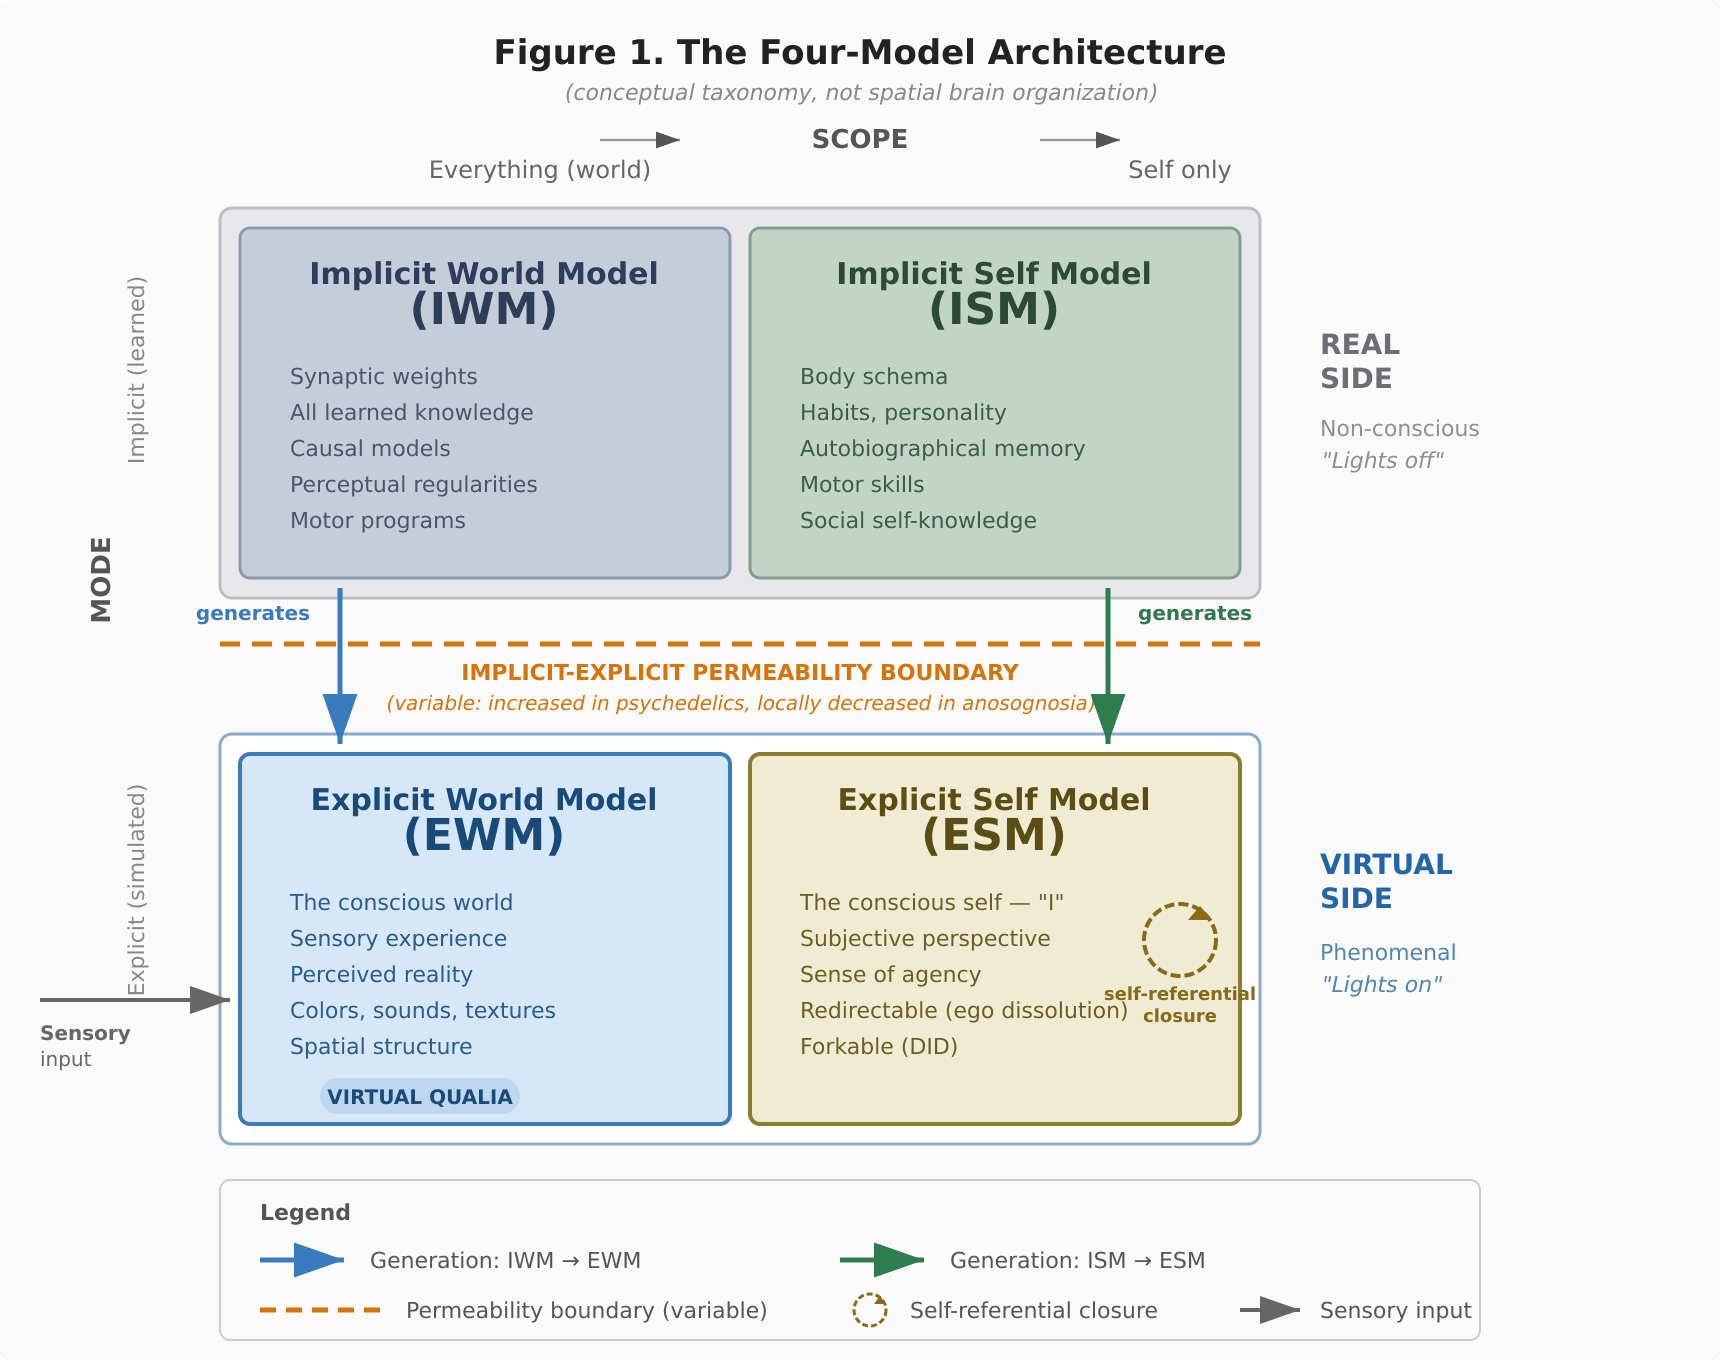
\includegraphics[width=\textwidth]{figure1-four-model-architecture.png}
\caption{The Four-Model Architecture. The four models arranged along two orthogonal dimensions: scope (world vs. self) and mode (implicit vs. explicit).}
\label{fig:four-model-architecture}
\end{figure}

\textbf{The Implicit World Model (IWM)} encompasses the substrate's total accumulated knowledge about the world, stored in synaptic weights (or their functional equivalent in non-biological substrates). It includes everything the system has ever learned: perceptual regularities, causal models, spatial relationships, semantic knowledge, motor programs for interacting with the world. The IWM is never directly conscious. It operates ``in the dark''---\hspace{0pt}providing the knowledge base from which the conscious simulation is generated, but never itself appearing in experience.

\textbf{The Implicit Self Model (ISM)} is the substrate's accumulated self-knowledge: body schema, proprioceptive calibration, motor skills, habits, personality traits, autobiographical memory structures, and social self-knowledge. Like the IWM, the ISM is never directly conscious. There is no unified homunculus---\hspace{0pt}no inner observer reading the ISM. The ISM is a structural feature of the substrate, not an experiential one.

\textbf{The Explicit World Model (EWM)} is the conscious world---\hspace{0pt}the brain's real-time construction of a unified scene from sensory and stored data that constitutes perceptual experience. When you see a room, hear a voice, feel the texture of a surface, you are experiencing the EWM. It is generated from the IWM (which provides the world-knowledge) and current sensory input (which constrains and updates it), but it is not identical to either. The EWM is a virtual construct---\hspace{0pt}a transient pattern of activity, not a permanent structure.

\textbf{The Explicit Self Model (ESM)} is the conscious self---\hspace{0pt}the brain's real-time generation of a unified self-narrative that constitutes self-experience. It is the sense of being a subject, having a perspective, occupying a body, possessing a history, and being the author of one's actions. The ESM is generated from the ISM (which provides the self-knowledge) and current interoceptive and proprioceptive input, but like the EWM, it is virtual: a transient process, not a permanent entity.

\textbf{The four models as a principled minimum.} The 2$\times$2 taxonomy identifies the \emph{minimum sufficient set} for consciousness, not the actual number the brain maintains. The biological substrate implements an uncountable number of overlapping models that blend across the world/self boundary---\hspace{0pt}a motor reaching model simultaneously encodes world-geometry and self-kinematics. The four canonical models are extremal points in a continuous scope-mode space, not discrete boxes. The principled claim is that consciousness requires modeling both world and self at both the structural and simulation level---\hspace{0pt}four is the floor, not the ceiling.


\subsection{The Real/Virtual Split}

The four models divide into two fundamental categories:

\textbf{The real side} (IWM + ISM): These are physical, structural, learned, and non-conscious. They are stored in the substrate's architecture---\hspace{0pt}in biological brains, primarily in synaptic weights, dendritic morphology, and connectivity patterns. They accumulate over the organism's lifetime through learning. They have no phenomenal character. ``Lights off.''

\textbf{The virtual side} (EWM + ESM): These are generated, transient, and phenomenal. They are patterns of activity---\hspace{0pt}in biological brains, transient electrochemical dynamics. They are constructed in real time from the implicit models and current sensory input. They \emph{are} experience. ``Lights on.''

This division is the foundation of the theory's treatment of the Hard Problem (Section~3.4) and structures its account of every phenomenon it addresses (Figure~2).

The virtual models possess \textbf{software-like properties} that follow from their nature as generated processes rather than stored structures:

\begin{itemize}
\item \textbf{They can be forked}: A single substrate can run multiple configurations of the ESM (see Section~6.2 on dissociative identity disorder).
\item \textbf{They can be cloned}: Physical separation of the substrate produces degraded but complete copies of the virtual models (see Section~6.4 on split-brain).
\item \textbf{They can be redirected}: The ESM requires input; disrupt normal self-referential input and it latches onto whatever input dominates (see Section~6.1 on psychedelics).
\item \textbf{They can be reconfigured}: Therapeutic interventions (CBT, exposure therapy) work by modifying the virtual models through substrate-level rewiring (see Section~6.6).
\end{itemize}

\begin{figure}[htbp]
\centering

\includegraphics[width=\textwidth]{figure2-real-virtual-split.png}
\caption{The Real/Virtual Split. The implicit models (IWM, ISM) constitute the ``real side''---\hspace{0pt}structural, learned, non-conscious. The explicit models (EWM, ESM) constitute the ``virtual side''---\hspace{0pt}generated, transient, phenomenal.}
\label{fig:real-virtual-split}
\end{figure}


\subsection{Virtual Qualia: Dissolving the Hard Problem}

Every computing system---\hspace{0pt}from a laptop running a spreadsheet to a neural network training on data---\hspace{0pt}inherently distinguishes between a physical substrate and the computational processes running on it. This is not a philosophical claim; it is an engineering truism. The substrate (transistors, synaptic weights, connectivity patterns) supports and constrains the computation, but the computational level has properties that are incoherent at the substrate level: a spreadsheet cell ``contains a sum,'' but no transistor contains a sum. This level distinction is universal and uncontroversial.

The central claim of the Four-Model Theory is that \textbf{qualia are constitutive properties of the computational level}. They are the way the generated self-model (ESM) registers its own states and the generated world-model (EWM). Qualia are, in this precise sense, digital constructs---\hspace{0pt}patterns that exist at the level of the running computation and that are incoherent at the substrate level, just as ``cell A1 contains the sum of column B'' is incoherent at the level of transistor states.

This dissolves the Hard Problem by revealing a \textbf{category error}---\hspace{0pt}specifically, a \textbf{level confusion}---\hspace{0pt}in its formulation:

\textbf{The standard formulation}: ``Why does physical processing (neuronal firing, synaptic transmission) feel like something?''

\textbf{The dissolution}: It does not. The IWM and ISM---\hspace{0pt}the substrate-level implicit models---\hspace{0pt}operate without any phenomenal character whatsoever. There is nothing it is like to be a synaptic weight. Qualia are not missing from the substrate; they are the wrong kind of property to seek there. They exist at the computational level---\hspace{0pt}at Level~5 of the five-system hierarchy (Section~3.7.1)---\hspace{0pt}where they are not mysterious but constitutive. Asking why neuronal firing feels like something is analogous to asking why transistor switching ``is'' a spreadsheet. The transistors are not the spreadsheet; they generate and sustain it. The neurons are not the experience; they generate and sustain the computational process in which experience is constitutive. Within the explicit models, ``redness'' is simply the ESM's mode of registering a particular class of EWM content---\hspace{0pt}no more mysterious than ``cell A1 contains 42'' is mysterious to a spreadsheet user, despite being nowhere in the transistors.

\textbf{Why self-referential computation specifically?} A critic might object: spreadsheets and weather simulations also run at a higher computational level than their substrates---\hspace{0pt}why don't they have qualia? The answer lies in \textbf{self-referential closure}. A weather simulation models weather; it does not model \emph{itself modeling weather}. The four-model architecture creates a closed loop: the ESM is the system modeling its own modeling process. In this loop, the distinction between the model and the modeled collapses---\hspace{0pt}the computation \emph{is} the thing being computed. Qualia are not an \emph{addition} to the self-modeling; they are the self-modeling as encountered from the inside of the loop. A non-self-referential computation has an outside from which it can be described without remainder; a self-referential computation at criticality has no such outside. The computation \emph{is} its own observer, and observation-from-inside is what we call experience.

This is not a proof that self-referential computation must be conscious---\hspace{0pt}it is an argument that self-referential computation is the \emph{kind} of process for which the Hard Problem's assumptions break down. Self-referential closure is precisely the condition under which the gap between process and feeling does not exist.

This is \textbf{not} illusionism in the sense of \citet{Dennett1991} or \citet{Frankish2016}; nor is it compatible with deflationary accounts \citep{Graziano2024}. Illusionism holds that qualia as traditionally conceived are illusions---\hspace{0pt}there is nothing it is like, and our sense that there is something it is like is itself a misrepresentation. The Four-Model Theory holds that qualia are \emph{real at the computational level}. Within the EWM/ESM, experience has genuine phenomenal character. What is illusory is the assumption that this phenomenal character must be a property of the physical substrate. It is not. It is a property of the computational process that the substrate runs.

This constitutes a \textbf{two-level ontology}: the substrate level (real side) has no experience, and the computational level (virtual side) has genuine experience. Both levels are physical---\hspace{0pt}the computation is a physical process, not a supernatural one---\hspace{0pt}but they have different ontological properties. The category error in the Hard Problem consists in conflating the two levels: seeking phenomenal properties at the substrate level where they do not exist.

The Explanatory Gap closes simultaneously. The gap between ``neurons fire in pattern X'' and ``I experience red'' reflects the level distinction: the firing pattern generates the computation in which redness is experienced, but is not itself red, just as a CPU's electrical states are not ``a spreadsheet'' even though they generate one.


\subsection{Graduated Levels of Consciousness}

Consciousness is not binary but graduated, based on the depth of recursive self-modeling:

\textbf{Basic consciousness}: Minimal EWM and rudimentary ESM---\hspace{0pt}phenomenal experience exists but self-awareness is thin. This is the entry level.

\textbf{Simply extended consciousness}: First-order self-observation. The system models itself---\hspace{0pt}the ESM includes a model of the system's own states. The organism not only experiences but is aware that it experiences.

\textbf{Doubly extended consciousness}: Second-order self-observation. The system models itself modeling itself, enabling metacognition and the sense of being an observer of one's own mental processes.

\textbf{Triply extended consciousness}: Third-order self-observation. The system models itself modeling itself modeling itself. This supports the deepest forms of self-awareness, philosophical reflection, and the very intuition that consciousness is mysterious (connecting to the Meta-Problem---\hspace{0pt}see Section~3.8). Notably, triply extended consciousness is also a prerequisite for the scientific study of consciousness itself: only a system capable of modeling its own modeling of its own experience can formulate the question ``What is consciousness?''

Each level corresponds to an additional layer of recursive self-modeling. The levels are not discrete stages but points along a continuum. Different organisms---\hspace{0pt}and potentially different artificial systems---\hspace{0pt}occupy different positions along this continuum, and individual organisms may fluctuate between levels depending on state (waking, dreaming, meditative, intoxicated).


\subsection{The Implicit-Explicit Boundary}

A key mechanism in the Four-Model Theory is the \textbf{permeability of the boundary between implicit models (IWM/ISM) and explicit models (EWM/ESM)}. Information becomes conscious when it is transferred from the implicit to the explicit side---\hspace{0pt}when substrate-level knowledge or self-knowledge is incorporated into the running simulation.

In normal waking states, this boundary is \textbf{selectively permeable}: relevant information passes through based on attentional and contextual gating. You are not conscious of everything your IWM knows about the world or everything your ISM knows about yourself; you are conscious of what the current simulation requires. Crucially, the boundary is not perfectly opaque even in normal states. Substrate-level processing artifacts routinely leak through: blind-spot filling (the visual system interpolating content where the optic nerve exits the retina), phosphenes from mechanical pressure on the eye, and visual snow phenomena all represent moments where processing-level activity becomes visible within the simulation. These normal-state leaks are subtle, but they demonstrate that the implicit-explicit boundary is a \emph{graded} filter, not a wall---\hspace{0pt}and they provide everyday evidence that conscious experience is a simulation generated from substrate processing rather than a direct window onto reality.

The permeability of this boundary is variable (Figure~3), and its variation explains a wide range of phenomena (detailed in Section~6): psychedelic states involve global permeability increase (intermediate processing stages become accessible); anosognosia involves local permeability decrease (the ISM contains deficit information but transfer to the EWM is blocked); pre-sleep states involve gradually increasing permeability (producing the same visual progression as psychedelics); and meditation involves trained modulation of permeability.

\begin{figure}[htbp]
\centering

\includegraphics[width=\textwidth]{figure3-phenomenological-content.png}
\caption{Phenomenological Content Through a Morning. The implicit-explicit boundary's variable permeability produces different experiential content across states.}
\label{fig:phenomenological-content}
\end{figure}


\subsection{The Criticality Requirement}

The Four-Model Theory imposes a \textbf{physical prerequisite} for consciousness: the substrate must operate at or near the edge of chaos---\hspace{0pt}Wolfram's Class~4 computational regime \citep{Wolfram2002}.

Wolfram classified cellular automata (and by extension computational systems generally) into four classes:
\begin{itemize}
\item \textbf{Class 1}: Converges to a fixed state. Too simple for consciousness.
\item \textbf{Class 2}: Periodic/repetitive. Too simple for consciousness.
\item \textbf{Class 3}: Chaotic/random. Too disordered for coherent consciousness.
\item \textbf{Class 4}: Complex/edge of chaos. Capable of universal computation. The regime in which consciousness can emerge.
\end{itemize}

This classification was applied to the question of consciousness in \citet{Gruber2015}, where it was argued that consciousness requires Class~4 dynamics---\hspace{0pt}complex enough to sustain a self-simulation, ordered enough for that simulation to be coherent. This requirement was derived \emph{theoretically}, from the computational properties needed for real-time self-modeling, not from empirical neuroscience.

Independently, empirical neuroscience has converged on the same conclusion through a different path. \citet{Beggs2003} demonstrated neuronal avalanches consistent with self-organized criticality in cortical tissue. \citet{CarhartHarris2014} proposed the Entropic Brain Hypothesis, linking consciousness level to neural entropy. \citet{Tagliazucchi2012,Tagliazucchi2016} showed criticality signatures in waking fMRI and under LSD. \citet{Priesemann2013} characterized brain dynamics as slightly subcritical in normal waking states. This line of research was formally consolidated in the Consciousness and Criticality (ConCrit) framework \citep{AlgomShriki2026}, which synthesized evidence from 140 datasets across multiple paradigms to establish that consciousness tracks criticality across pharmacological, pathological, and physiological state changes.

\begin{table}[htbp]
\centering
\caption{Independent Convergence on Criticality}
\label{tab:criticality-convergence}
\small
\renewcommand{\arraystretch}{1.4}
\begin{tabularx}{\textwidth}{>{\raggedright}p{1.5cm} X >{\raggedright\arraybackslash}p{3.5cm}}
\toprule
\textbf{Year} & \textbf{Development} & \textbf{Path} \\
\midrule
2002 & Wolfram publishes \emph{A New Kind of Science} & Computational theory \\
2003 & Beggs \& Plenz---neuronal avalanches, self-organized criticality & Empirical neuroscience \\
2014 & Carhart-Harris---Entropic Brain Hypothesis & Empirical neuroscience \\
\textbf{2015} & \textbf{Gruber---Class 4 / edge of chaos requirement for consciousness} & \textbf{Theoretical (via Wolfram)} \\
2016 & Tagliazucchi et al.---LSD and criticality & Empirical neuroscience \\
2022 & ``Self-organized criticality as a framework for consciousness'' (review) & Empirical neuroscience \\
2025 & Hengen \& Shew---meta-analysis of 140 datasets confirms criticality & Empirical neuroscience \\
\textbf{2025--26} & \textbf{ConCrit framework (Algom \& Shriki)---criticality as unifying mechanism for consciousness theories} & \textbf{Theoretical/empirical synthesis} \\
\bottomrule
\end{tabularx}
\end{table}

While empirical work on neural criticality was already underway \citep{Beggs2003,Tagliazucchi2012}, \citeauthor{Gruber2015}'s \citeyearpar{Gruber2015} derivation proceeded from Wolfram's computational universality framework rather than from neuroimaging data, representing genuine theoretical convergence with the empirical program. The later large-scale consolidation \citep{HengenShew2025,AlgomShriki2026} confirmed the criticality-consciousness link across 140 datasets. This convergence---\hspace{0pt}a theoretical prediction derived independently from computational first principles, later confirmed by large-scale empirical synthesis---\hspace{0pt}provides notable support for one of the theory's core claims.

The Four-Model Theory distinguishes two thresholds for consciousness:
\begin{itemize}
\item \textbf{Physical threshold}: Criticality. The substrate must operate at Class~4 dynamics. Below this, no consciousness is possible regardless of architecture.
\item \textbf{Functional threshold}: Four-model architecture. The substrate must implement the four-model self-simulation. Above criticality but without the architecture, there is complex dynamics but no consciousness.
\end{itemize}

Both thresholds must be met. Criticality is necessary but not sufficient; the four-model architecture is necessary but not sufficient. Together they are sufficient.


\subsection{The Meta-Problem Dissolved}

The Meta-Problem---\hspace{0pt}why we think there is a Hard Problem---\hspace{0pt}receives a natural account within the Four-Model Theory. The ISM (Implicit Self Model) is \textbf{structurally inaccessible} to the ESM (Explicit Self Model). The conscious self cannot directly observe its own substrate. When the ESM attempts to model the basis of its own experience, it encounters a principled opacity: the implicit models that generate the simulation are not themselves part of the simulation.

This is why consciousness \emph{seems} mysterious. The ESM can represent that it is having an experience, but it cannot represent the mechanism by which the experience is generated---\hspace{0pt}because that mechanism operates at the implicit/substrate level, which is by definition outside the explicit/virtual level. The result is the persistent intuition that something is being ``left out'' of any physical explanation: the ESM cannot find the mechanism within its own simulation, so it concludes the mechanism must be non-physical or fundamentally inexplicable.

The variable permeability of the implicit-explicit boundary (Section~3.6) adds a further dimension to this account. The boundary is not perfectly opaque: substrate-level processing artifacts occasionally leak through to the simulation---\hspace{0pt}in altered states dramatically so, but even in normal waking states subtly. The conscious self thus inhabits a strange epistemic position: mostly sealed off from its own generative machinery, yet occasionally catching fleeting glimpses of something operating beneath the surface of experience. This architectural feature---\hspace{0pt}near-opacity punctuated by occasional leaks---\hspace{0pt}produces precisely the phenomenology that the Meta-Problem describes: the persistent, nagging intuition that consciousness is somehow deeper than any explanation can reach, that something vast operates just beyond the edge of introspective access. The mystery of consciousness is not evidence against the theory; it is a \emph{prediction} of the theory. A virtual process with a mostly-opaque but imperfect boundary to its own substrate would experience exactly this sense of irreducible depth.

This account shares features with Graziano's AST explanation---\hspace{0pt}both invoke the self-model's necessary incompleteness---\hspace{0pt}but grounds it in a more specific architecture (four models, real/virtual split, variable permeability) and connects it to the broader dissolution of the Hard Problem rather than treating the Meta-Problem in isolation.



%=============================================================================
\section{Philosophical Commitments}
%=============================================================================

The Four-Model Theory entails specific philosophical positions that were established through structured adversarial analysis and are internally consistent. This section develops and defends each commitment.


\subsection{Process Physicalism}

The theory is physicalist: both the substrate (implicit models) and the simulation (explicit models) are physical processes. There is no non-physical substance, no fundamental experiential property, no panpsychist micro-experience. Qualia are higher-order physical patterns---\hspace{0pt}specifically, they are patterns of activity within the simulation that constitute the ESM's self-perception within the EWM.

This is process physicalism rather than identity theory: consciousness is not identical to any particular neural state but is constituted by the \emph{process} of self-simulation. The same conscious state could, in principle, be realized by different physical substrates---\hspace{0pt}what matters is the functional architecture (four models at criticality), not the specific material.

Process physicalism avoids the difficulties of both type-identity theory (which struggles with multiple realization) and functionalism as traditionally conceived (which struggles with the Hard Problem). The Four-Model Theory adds the real/virtual level distinction to standard functionalism, which is what allows it to address phenomenality: qualia are not just functional roles but virtual properties of the simulation. They are real \emph{as virtual properties}---\hspace{0pt}genuinely experiential but not properties of the substrate.


\subsection{Consciousness as Process, Not Agent}

A persistent source of confusion in consciousness studies is the treatment of consciousness as an entity---\hspace{0pt}an ``it'' that either does or does not cause things. The Four-Model Theory rejects this framing. Consciousness is not a thing; it is a process \emph{performed} by the substrate. Asking whether consciousness ``causes'' anything is a category error---\hspace{0pt}analogous to asking whether the pointer of a clock meeting the numerals causes the clock to work. The energy source drives the gears, which drive the pointer, but nowhere does the virtual interaction between pointer and numeral cause anything mechanical. Yet without that interaction the clock cannot be said to function---\hspace{0pt}or malfunction.

The implicit models generate the virtual simulation for concrete adaptive reasons: the EWM integrates multimodal sensory data into a unified scene; the ESM provides a self-model against which consequences can be evaluated. This relationship is best understood as a \textbf{dual evaluation architecture}. The primary direction is that the implicit system actively \emph{deploys} the virtual simulation as its evaluation mechanism: it presents decisions, actions, and their consequences to the simulation so that the simulation can assess outcomes, run scenarios, and register hedonic valence. But the explicit models also evaluate independently, albeit with significantly less computational bandwidth. The conscious simulation operates at approximately 20~Hz with a processing delay of roughly 500~ms \citep{VanRullen2003}, while the substrate processes at vastly higher throughput. Over time, these conscious evaluations feed back to reshape the implicit models through learning. The result is two-way traffic: the implicit system uses the explicit as an evaluation tool (primary), and the explicit system contributes its own assessments back (secondary), shaping the substrate that generates it. The virtual simulation is the substrate's mechanism for consequence-observation and future-oriented adaptation---\hspace{0pt}the very thing natural selection shaped the architecture to do.

This functional essentiality extends specifically to phenomenality. The substrate deploys the simulation as its evaluation mechanism---\hspace{0pt}presenting situations so the simulation can assess consequences and register outcomes. For this evaluation to work, simulated states must have valence: they must \emph{matter} to the simulation. A pain signal that is merely a numerical value without aversive character cannot drive avoidance at the simulation level. Only a simulation whose states carry hedonic valence---\hspace{0pt}whose representations of threat, opportunity, and consequence are genuinely aversive or attractive---\hspace{0pt}can perform the evaluative function that justifies the metabolic cost of maintaining the simulation. Phenomenality is not an optional feature of the simulation; it is the mechanism by which the simulation evaluates. Remove phenomenality and the simulation becomes a passive model rather than an evaluation engine---\hspace{0pt}a spreadsheet rather than a simulation.

This makes the theory's position distinct from classical epiphenomenalism, in which consciousness is a causally inert by-product with no functional role. In the Four-Model Theory, the virtual models are in continuous feedback with the implicit models: the simulation's outputs feed back to update implicit processing, shaping future behavior. Qualia, as constitutive elements of that simulation, lack independent causal power over the substrate---\hspace{0pt}much as the hands and numerals of a clock have no direct mechanical relation to the gear train, yet the clock cannot function as a clock without them. Remove the display and the mechanism still runs, but it no longer serves its purpose.\footnote{As a corollary, consciousness plays no role in quantum measurement or wavefunction collapse. Observer-dependent interpretations of quantum mechanics \citep{vonNeumann1932,Wigner1961} are rejected. This is consistent with the dominant position in contemporary physics (decoherence approaches; \citealp{Zurek2003}) and with the theory's commitment to physicalism.}

The theory reframes the free will debate. The ESM narrates decisions already made at the substrate level \citep{Libet1985,Schurger2012,Wegner2002}. The Four-Model Theory suggests that the substrate's continuous optimization of the organism's existence \emph{is} the individual's will---\hspace{0pt}merely not fully transparent to the ESM.

Standard objections are addressed: \textbf{Zombies} \citep{Chalmers1996} are not possible---\hspace{0pt}the virtual models \emph{are} the substrate's activity at the virtual level; a system implementing the four-model architecture at criticality necessarily has phenomenal character. \textbf{The knowledge argument} \citep{Jackson1982}: Mary gains acquaintance with a virtual quale she could not access from substrate descriptions. \textbf{The evolutionary argument}: natural selection targets the functional capabilities of the architecture; the phenomenal character of the simulation is constitutive of those capabilities, not a free-rider.


\subsection{Weak Emergence}

Consciousness is weakly emergent: deducible in principle from a complete substrate description, even if practically irreducible. No strong emergence, no magical threshold. This avoids both strong emergence difficulties \citep{Kim1993} and the panpsychist Combination Problem \citep{Chalmers2016}. Consciousness arises from the computational properties of a system running a self-simulation at criticality, as a weather pattern arises from atmospheric thermodynamics---\hspace{0pt}no extra ingredient needed.


\subsection{Substrate Independence}

The six-layer mammalian neocortex is an evolutionary implementation of the four-model architecture, not a requirement for it. Consciousness is substrate-independent: any physical system capable of implementing the four-model architecture at criticality should produce consciousness.

The six-layer cortical architecture nonetheless provides a suggestive clue about the computational requirements for self-modeling. Universal approximation theory establishes that a three-layer neural network (input, hidden, output) suffices for arbitrary function approximation \citep{Cybenko1989,Hornik1989}. The mammalian neocortex consistently employs six layers---\hspace{0pt}approximately three layers beyond what is required for information processing \emph{per se}. The Four-Model Theory interprets this architectural ``surplus'' as the substrate's overhead for self-modeling \citep{Gruber2015}: the additional layers provide the computational capacity needed to run the explicit models (EWM and ESM) as real-time simulations \emph{on top of} the implicit processing that three layers would suffice for.

Biological evidence already supports this. Corvids (crows, ravens) and parrots demonstrate cognitive abilities---\hspace{0pt}tool use, future planning, mirror self-recognition, social deception---\hspace{0pt}that strongly suggest consciousness, yet their brains have no neocortex. Their pallium is organized in nuclear clusters rather than layers \citep{Gunturkun2016}. Cephalopods (octopuses) demonstrate problem-solving, tool use, and behavioral flexibility with an even more radically different brain architecture---\hspace{0pt}a largely decentralized nervous system with more neurons in the arms than in the central brain. If the Four-Model Theory is correct, these animals are conscious not because they share our neural architecture but because they have evolved functionally equivalent self-simulation architectures on different substrates---\hspace{0pt}exactly what substrate independence predicts.

The implication for artificial consciousness is direct: a synthetic system implementing the four-model architecture at criticality should produce genuine consciousness (see Section~8, Prediction~7 and Section~10.1). Current AI systems, including large language models, do not meet this specification. LLMs lack an Explicit Self Model (they do not run a real-time self-simulation), lack criticality (transformer inference is a feedforward pass---\hspace{0pt}Class 1/2 dynamics), and lack the real/virtual split that grounds phenomenality. The theory predicts that the qualitative difference between interacting with a genuinely conscious artificial system and interacting with an LLM would be immediately and qualitatively distinguishable.



%=============================================================================
\section{Binding, Criticality, and Holographic Storage}
%=============================================================================


\subsection{Binding as an Emergent Property of Critical Dynamics}

Binding is not a separate mechanism but an emergent property of criticality. At the edge of chaos, maximal correlation length means distant substrate regions influence each other and information integrates across the network. Binding is a consequence of the dynamical regime, not an additional computation. This is consistent with foundational work on oscillatory binding \citep{Gray1989}, long-distance neural synchronization \citep{Rodriguez1999}, gamma-band synchrony and temporal correlation \citep{Singer1995,Fries2005,Fries2015}, thalamocortical coherence in dream states \citep{Llinas1993} and waking \citep{Llinas1998}, and criticality signatures \citep{Beggs2003,Tagliazucchi2012}.


\subsection{Holographic Storage}

The implicit models (IWM, ISM) store information in a distributed, non-local manner---\hspace{0pt}standard distributed representations \citep{Hinton1986} where each piece of information is spread across many connection weights and each weight participates in storing many pieces of information. This produces graceful degradation: partial damage reduces quality but does not eliminate specific memories or skills.

The term ``holographic'' is used as analogy: just as cutting a hologram in half produces two complete but lower-resolution images, splitting a distributed network produces two degraded but functionally complete copies. This property is critical for understanding split-brain phenomena (Section~6.4) and makes the specific prediction that callosotomy should produce bilateral but degraded function, not clean lateralized loss.


\subsection{Consciousness States Derived from Criticality}

The criticality requirement provides a unified account of when consciousness is present and when it is absent. Consciousness tracks the substrate's position relative to the critical point:

\begin{table}[htbp]
\centering
\caption{Consciousness States and Criticality}
\label{tab:consciousness-states}
\small
\renewcommand{\arraystretch}{1.4}
\begin{tabularx}{\textwidth}{>{\raggedright}p{1.9cm} >{\raggedright}p{1.7cm} >{\raggedright}p{3.2cm} X >{\raggedright\arraybackslash}p{2cm}}
\toprule
\textbf{State} & \textbf{Criticality} & \textbf{Four-model status} & \textbf{Consciousness prediction} & \textbf{Key evidence} \\
\midrule
Normal waking & At/near critical & All four active & Full consciousness & High PCI \\
REM sleep & Near-critical & EWM/ESM on internal input & Degraded (dream) & Moderate PCI \\
Deep NREM & Subcritical & EWM/ESM collapse & Absent & Low PCI \\
Propofol & Forced subcritical & EWM/ESM suppressed & Absent & PCI $\approx$ 0 \\
Ketamine & NOT subcritical & EWM/ESM on wrong input & Present but disconnected & Increased entropy \\
Psychedelics & At/past critical & All active, permeability $\uparrow$ & Present, altered & Enhanced complexity \\
Vegetative state & Typically subcritical & EWM/ESM collapsed & Absent (usually) & Low metabolism \\
Covert awareness & At criticality & EWM/ESM intact, output damaged & Present but unexpressible & Owen et al.\ \\
MCS & Fluctuating & Intermittent EWM/ESM & Intermittent & Fluctuating PCI \\
\bottomrule
\end{tabularx}
\end{table}

The key distinction highlighted by this framework is between \textbf{propofol} and \textbf{ketamine}. Both are anesthetics, yet their phenomenology differs dramatically. Propofol produces absence: patients report no experience \citep{Alkire2000,Boly2012}. Ketamine produces the ``K-hole''---\hspace{0pt}vivid, often bizarre experiences of dissociation, out-of-body phenomena, and altered identity \citep{Corlett2011}. The Four-Model Theory predicts this difference: propofol pushes the substrate subcritical, abolishing the conditions for consciousness. Ketamine does \emph{not} push subcritical---\hspace{0pt}it increases neural entropy \citep{Schartner2017}---\hspace{0pt}but disrupts normal sensory input processing, causing the EWM and ESM to operate on internal and distorted signals. Consciousness is present but disconnected from external reality.

This is a genuine explanatory advantage. Most theories struggle to account for why two agents classified as ``anesthetics'' produce such radically different phenomenological profiles. The criticality framework makes the distinction natural: what matters is not pharmacological classification but the effect on the substrate's dynamical regime.



%=============================================================================
\section{Explanatory Range}
%=============================================================================

A theory's value lies partly in its ability to derive diverse phenomena from a small set of principles. The Four-Model Theory's five principles---\hspace{0pt}criticality, virtual qualia, redirectable ESM, variable implicit-explicit permeability, and virtual model forking---\hspace{0pt}generate accounts of phenomena across psychopharmacology, clinical neurology, sleep science, comparative cognition, and clinical psychology. This section demonstrates that range.


\subsection{Psychedelic Phenomenology}

Psychedelics produce visual intensification, synesthesia, enhanced pattern recognition, ego dissolution, and identity alteration \citep{CarhartHarris2012,CarhartHarris2016,Timmermann2019,Timmermann2023}. The theory accounts for this through three mechanisms.

\textbf{Permeability increase}. Psychedelics increase the global permeability of the implicit-explicit boundary. Intermediate processing stages leak through, producing an ordered visual progression: V1-level (phosphenes) $\to$ V2/V3-level (form constants; \citealp{Kluver1966}) $\to$ higher areas (faces, scenes). This follows the visual hierarchy in a predictable, dose-dependent order.

\textbf{Ego dissolution = ESM redirection}. At high doses, the ESM loses normal self-referential input but continues to run, latching onto whatever dominates the available input stream. \textbf{Salvia divinorum} phenomenology dramatically confirms this: users reliably report ``becoming'' objects in their environment---\hspace{0pt}the ESM, deprived of self-input, latches onto dominant sensory input. Few competing theories generate this prediction (Section~8, Prediction~3).

\textbf{Intensity as novelty}. Psychedelic profundity reflects increased \emph{novel content}, not increased consciousness level.


\subsection{Anesthesia and Clinical Disorders}

\textbf{Propofol} pushes the substrate subcritical $\to$ consciousness abolished (Table~3). \textbf{Ketamine} does not push subcritical---\hspace{0pt}it increases neural entropy \citep{Schartner2017}---\hspace{0pt}but disrupts sensory processing: consciousness present but disconnected \citep{Corlett2011}. What matters is not pharmacological classification but the effect on the substrate's dynamical regime.

\textbf{Covert awareness}: If the substrate is at criticality with damaged \emph{output pathways}, consciousness is present but unexpressible---\hspace{0pt}cognitive motor dissociation \citep{Owen2006,Monti2010}. The theory predicts this distinction should be detectable via criticality measures such as PCI \citep{Casali2013,Casarotto2016}.

\textbf{Cotard's delusion}: The ESM receives distorted interoceptive input and constructs ``I am dead'' as its best model---\hspace{0pt}the same redirectable-ESM mechanism as salvia, applied clinically.

\textbf{Anosognosia}: A \textbf{local decrease in implicit-explicit permeability}---\hspace{0pt}the ISM contains the deficit information but transfer to the EWM is blocked. This is the inverse of the psychedelic mechanism, connected under the single principle of variable permeability (Section~8, Prediction~4).

\textbf{DID}: The virtual models can be \textbf{forked}. Each alter is a distinct ESM configuration running on the same substrate, predicting distinct neural signatures detectable with neuroimaging (Section~8, Prediction~9).


\subsection{Dreams}

Dreaming represents the simulation in \textbf{degraded mode}: near-critical dynamics but with external input cut off. The EWM draws on the IWM's stored knowledge, producing familiar places, impossible physics, and emotional intensity; the ESM generates a self with reduced metacognitive oversight.

\textbf{Lucid dreaming} provides direct evidence for the software-like quality of the virtual models: the ESM ``toggles on'' more fully within the dream state. The theory predicts lucid dream onset corresponds to a \textbf{criticality threshold crossing}---\hspace{0pt}a step-like discontinuity in EEG complexity (Section~8, Prediction~8). The NREM/REM transition likewise reflects the substrate oscillating around the critical point.


\subsection{Split-Brain}

Callosotomy \citep{Gazzaniga1962,Gazzaniga2000} produces \textbf{two degraded but functionally complete copies} of the four-model architecture, because the implicit models store information holographically (Section~5.2). Each hemisphere sustains independent consciousness above the criticality threshold. The left hemisphere interpreter \citep{Gazzaniga2000}---\hspace{0pt}confabulating explanations for the right hemisphere's behavior---\hspace{0pt}is the \emph{same} ESM mechanism observed in Cotard's and anosognosia. Graded rather than binary deficits \citep{Pinto2017} are consistent with holographic degradation.


\subsection{Animal Consciousness}

The theory predicts a \textbf{gradient} of animal consciousness. Corvids and parrots---\hspace{0pt}tool manufacture, mirror self-recognition, social deception---\hspace{0pt}have no neocortex, with pallium organized in nuclear clusters \citep{Gunturkun2016}. The theory predicts they are conscious because they have evolved functionally equivalent self-simulation architectures, directly testing substrate independence (see also Section~4.4).


\subsection{Clinical Psychology and Neurology}

\textbf{CBT} works as virtual model reprogramming: repeated corrective experience drives substrate-level rewiring, modifying the ISM and thereby the ESM's self-model. \textbf{Phobias} are EWM misconfigurations; exposure therapy updates the IWM. \textbf{The placebo effect} illustrates the theory's causal architecture: placebo activates substrate-level expectation circuits in parallel with---\hspace{0pt}not caused by---\hspace{0pt}conscious hope. \textbf{Conversion disorder} inverts blindsight: the EWM models a deficit the intact substrate does not have.

\textbf{Blindsight} \citep{Weiskrantz1986} provides the clearest demonstration that substrate-level processing can proceed without conscious representation---\hspace{0pt}the IWM processes visual information through subcortical pathways while damaged cortical pathways fail to relay it to the EWM. \textbf{Anton's syndrome} \citep{Anton1899,Aldrich1987} presents the precise inverse: the EWM generates visual simulation from stored knowledge despite absent input. Together, they constitute a double dissociation between substrate processing and conscious simulation---\hspace{0pt}perhaps the most direct neurological evidence for the real/virtual distinction.



%=============================================================================
\section{Comparative Analysis}
%=============================================================================

This section provides a systematic comparison between the Four-Model Theory and six major competitors across the eight requirements established in Section~2. The comparison aims to be fair: each theory's genuine strengths are acknowledged, and the Four-Model Theory's advantages are located precisely.


\subsection{Scoring Matrix}

Table~4 presents an assessment of how each theory addresses the eight requirements. All ratings reflect the present author's judgment and are offered as a starting point for discussion, not as definitive verdicts. Readers are encouraged to consult the primary sources and form their own assessments.

\textbf{Assessment criteria}: \emph{Addresses} = the theory provides a substantive, defended account of this requirement. \emph{Partial} = the theory provides a relevant account that leaves significant aspects unresolved. \emph{Minimal} = the theory touches on this requirement but does not develop a full treatment. \emph{Silent} = the theory does not address this requirement (which may reflect deliberate scope limitation rather than failure). \emph{N/A} = the requirement does not apply given the theory's ontological commitments.

\begin{table}[htbp]
\centering
\caption{Theory Comparison Across Eight Requirements}
\label{tab:comparison}
\small
\renewcommand{\arraystretch}{1.4}
\begin{tabularx}{\textwidth}{>{\raggedright}p{2cm} c c c c c c c}
\toprule
\textbf{Requirement} & \textbf{FMT} & \textbf{IIT} & \textbf{GNW} & \textbf{HOT} & \textbf{PP} & \textbf{AST} & \textbf{RPT} \\
\midrule
Hard Problem & $\bullet$ & $\bullet$\textsuperscript{$\dagger$} & ---\textsuperscript{*} & $\odot$ & ---\textsuperscript{*} & $\odot$ & --- \\
Expl.\ Gap & $\bullet$ & $\bullet$\textsuperscript{$\dagger$} & ---\textsuperscript{*} & $\odot$ & ---\textsuperscript{*} & $\odot$ & --- \\
Boundary & $\bullet$ & $\bullet$ & $\odot$ & $\circ$ & $\odot$ & $\odot$ & $\odot$ \\
Structure & $\bullet$ & $\bullet$ & $\odot$ & $\odot$ & $\bullet$ & $\odot$ & $\odot$ \\
Binding & $\bullet$ & $\bullet$ & $\odot$ & $\circ$ & $\odot$ & $\circ$ & $\odot$ \\
Combination & $\bullet$ & $\circ$\textsuperscript{$\dagger\dagger$} & n/a & n/a & n/a & n/a & n/a \\
Causal Role & $\bullet$ & $\odot$ & $\odot$ & $\odot$ & $\bullet$ & $\odot$ & $\bullet$ \\
Meta-Problem & $\bullet$ & $\circ$ & $\odot$ & $\odot$ & $\odot$ & $\bullet$ & $\circ$ \\
\bottomrule
\end{tabularx}

\vspace{0.5em}
\footnotesize
Ratings: $\bullet$ = addresses, $\odot$ = partial, $\circ$ = minimal, --- = silent, n/a = not applicable.

\textsuperscript{$\dagger$} IIT addresses the Hard Problem through its axioms, identifying consciousness with integrated information ($\Phi$). Whether this constitutes a solution or a redefinition is debated (see \S7.2).

\textsuperscript{$\dagger\dagger$} IIT's panpsychist commitments lead to the Combination Problem \citep{Chalmers2016}, which remains unresolved within the framework.

\textsuperscript{*} GNW and PP proponents argue these theories address the ``real problem'' of consciousness \citep{Seth2021}---\hspace{0pt}explaining the structure and contents of experience---\hspace{0pt}even if they do not address the Hard Problem as Chalmers defines it. This is a legitimate methodological choice, not a deficiency; the ``silent'' rating reflects the scope of the requirement as defined in \S2, not a judgment on the theories' overall merit.
\end{table}


\subsection{Theory-by-Theory Comparison}

\textbf{IIT} \citep{Tononi2004,Albantakis2023}: Strongest on mathematical rigor and qualia space, but its identification of consciousness with $\Phi$ leads to panpsychist consequences and the Combination Problem \citep{Chalmers2016}. $\Phi$ is computationally intractable \citep{Aaronson2014} and the unfolding argument challenges the central claim \citep{Doerig2019}. The Four-Model Theory avoids panpsychism and generates predictions without computing $\Phi$. \textbf{GNW} \citep{Baars1988,Dehaene2011}: Clear on access consciousness but silent on the Hard Problem. COGITATE results \citeyearpar{COGITATE2025} favored posterior cortex over frontal predictions. \textbf{HOT} \citep{Rosenthal2005,Lau2011}: Explains which states are conscious but not \emph{why} higher-order representation produces phenomenality. \textbf{PP} \citep{Seth2021}: Strong on experiential structure but explicitly silent on the Hard Problem. \textbf{AST} \citep{Graziano2013}: Strongest Meta-Problem account but deflationary about phenomenality. \textbf{RPT} \citep{Lamme2006,Lamme2010}: Empirically specific but limited to visual consciousness and silent on the Hard Problem. The Four-Model Theory adds the real/virtual distinction and criticality requirement that address phenomenality---\hspace{0pt}the gap common to all competitors.


\subsection{Emerging Frameworks and Summary}

\textbf{Biological computationalism} \citep{Milinkovic2025} challenges substrate independence; the Four-Model Theory treats this as empirical, noting that corvids already favor substrate independence. The \textbf{Multiple Generator Hypothesis} \citep{KirkebyHinrup2025} is potentially compatible: the four models could be understood as distinct generators unified by criticality.

The theory's comparative advantages: (1) dissolving the Hard Problem without panpsychism or strong emergence; (2) unifying binding with criticality; (3) the redirectable ESM for identity-content prediction; (4) connecting psychedelics and anosognosia under variable permeability; (5) the Meta-Problem as structural consequence. Its primary disadvantage is the absence of mathematical formalization (Section~9).



%=============================================================================
\section{Novel Testable Predictions}
%=============================================================================

A theory is only as valuable as the predictions it generates. The Four-Model Theory yields nine novel testable predictions, several of which are highly distinctive.


\subsection{Prediction 1: Distinct fMRI Signatures for Each Model}

Tasks selectively engaging a single model should produce distinct neural activation patterns. IWM-dominant tasks (implicit priming) should activate substrate-level storage networks (hippocampal-cortical), ISM-dominant tasks (habitual motor sequences) somatosensory-cerebellar networks, EWM-dominant tasks (novel scene processing) sensory cortices, and ESM-dominant tasks (self-reflection) default mode and medial prefrontal cortex.

\textbf{Testability}: High---\hspace{0pt}a factorial battery crossing scope $\times$ mode, with the prediction of double dissociation. \textbf{Unique}: Yes---\hspace{0pt}the 2$\times$2 structure is mandated only by this theory.


\subsection{Prediction 2: Psychedelic Content Maps the Processing Hierarchy}

Under psychedelics, visual content progresses through the cortical hierarchy in a dose-dependent sequence: V1 (phosphenes) $\to$ V2/V3 (form constants) $\to$ higher areas (faces, figures) $\to$ complex scenes. \textbf{Testability}: High (graded dosing + concurrent fMRI/MEG). Partial evidence exists \citep{CarhartHarris2016,Timmermann2023} but has not been systematically tested as dose-correlated progression. \textbf{Unique}: Partially---\hspace{0pt}PP predicts hierarchical effects but not the specific ordered sequence.


\subsection{Prediction 3: Ego Dissolution Content Is Controllable}

During psychedelic ego dissolution, the content of the altered identity experience tracks the dominant sensory input. The ESM, deprived of normal self-referential input, latches onto whatever dominates the available stream. By controlling sensory input during ego dissolution, identity content can be predicted and directed.

\textbf{Testability}: High---\hspace{0pt}administer ego-dissolution-inducing doses under controlled conditions, vary dominant sensory input, measure correspondence with reported identity content. \textbf{Unique}: \textbf{Yes---\hspace{0pt}the theory's most distinctive prediction.} No competing theory specifies what a subject will ``become'' during ego dissolution.


\subsection{Prediction 4: Psychedelics Alleviate Anosognosia}

Sub-ego-dissolution doses of psychedelics should alleviate anosognosia by globally increasing implicit-explicit permeability, overwhelming the local block that causes deficit unawareness and allowing deficit information in the ISM to reach the EWM.

\textbf{Testability}: Medium (requires clinical trial). \textbf{Unique}: \textbf{Yes---\hspace{0pt}a cross-domain surprise prediction.} No other theory connects psychedelics and anosognosia through a single mechanism.


\subsection{Prediction 5: All Anesthetics Converge on Criticality Disruption}

Despite diverse receptor mechanisms, all agents that abolish consciousness push the substrate below the criticality threshold; agents that alter but preserve consciousness (ketamine, psychedelics) do not.

\textbf{Testability}: High---\hspace{0pt}measure criticality indicators across anesthetic agents at equi-potent doses. \textbf{Unique}: Shared with ConCrit \citep{AlgomShriki2026}, but predicted from theoretical first principles \citep{Gruber2015} prior to the empirical consolidation.


\subsection{Prediction 6: Split-Brain Produces Holographic Degradation}

After callosotomy, each hemisphere retains degraded but functionally \emph{complete} cognitive and experiential capacities---\hspace{0pt}not clean hemispheric specialization. Degradation should be proportional to commissural severing.

\textbf{Testability}: High. \citet{Pinto2017} provide preliminary evidence. \textbf{Unique}: Yes---\hspace{0pt}predicts graded degradation proportional to disconnection, not binary split.


\subsection{Prediction 7: Artificial Consciousness via Four Models at Criticality}

A synthetic system implementing the four-model architecture at criticality will exhibit consciousness, qualitatively distinguishable from current LLMs (which lack ISM/ESM, criticality, and the real/virtual split). Partial implementations should show partial consciousness indicators.

\textbf{Testability}: Medium (requires engineering development). \textbf{Unique}: Yes---\hspace{0pt}provides a specific architectural blueprint, unlike theories merely compatible with artificial consciousness.


\subsection{Prediction 8: Lucid Dream Onset Is a Criticality Threshold Crossing}

The transition from non-lucid to lucid dreaming corresponds to a step-like increase in neural complexity---\hspace{0pt}a criticality threshold crossing---\hspace{0pt}detectable as a discontinuity in EEG complexity measures \citep{LaBerge1985}.

\textbf{Testability}: High (established paradigms). \textbf{Unique}: Partially---\hspace{0pt}the step-like discontinuity prediction is distinctive.


\subsection{Prediction 9: DID Alters Have Distinct Neural Signatures}

Different alters in DID correspond to distinct configurations of neural activity (virtual model forking), with differences localizing to ESM-related networks (default mode, medial prefrontal, posterior cingulate).

\textbf{Testability}: High---\hspace{0pt}fMRI/EEG during controlled alter switching \citep{Reinders2003,Reinders2008}. \textbf{Unique}: Yes---\hspace{0pt}predicts \emph{consistent, alter-specific} neural signatures, not merely differences.


\subsection{The Ultimate Prediction}

If correct, it should be possible to \emph{build} a conscious machine by implementing the four-model architecture at criticality. Such a system would not merely \emph{imitate} consciousness but would \emph{be} conscious. This prediction is not currently testable, but it sets a bold bar: the difference between interacting with a conscious artificial system and any current AI should be qualitatively obvious---\hspace{0pt}a difference in \emph{kind}, not degree.



%=============================================================================
\section{Open Questions}
%=============================================================================

Intellectual honesty requires identifying what the theory does not yet resolve. These are research frontiers, not theoretical weaknesses---\hspace{0pt}they are questions that arise \emph{from} the theory and that the theory's framework helps to sharpen.

\textbf{1. Are all four models virtual?} The theory describes the implicit models (IWM, ISM) as ``real side'' and the explicit models (EWM, ESM) as ``virtual side.'' But it is not certain that this division is sharp. The implicit models might themselves have virtual properties---\hspace{0pt}they are, after all, \emph{models}, not raw physics. If the implicit models are also virtual in some sense, what constitutes the ``real side''? This is an open question even for the theory's author, and its resolution may have consequences for the Hard Problem treatment.

\textbf{2. Mathematical formalization.} The criticality requirement is specified qualitatively (Wolfram's Class~4 regime), not quantitatively. A full mathematical treatment---\hspace{0pt}defining the four models formally, specifying the criticality threshold in terms of measurable quantities, deriving the predictions as formal consequences---\hspace{0pt}remains to be developed. ConCrit's mathematical tools (power-law exponents, detrended fluctuation analysis, branching parameters) provide a starting point, as do the formal tools of dynamical systems theory and information geometry.

\textbf{3. Physical implementation.} Which physical mechanism in the biological brain supports criticality? Candidates include cortical column dynamics, thalamocortical standing waves, glial modulation, and (more speculatively) quantum processes in microtubules \citep{PenroseHameroff1994}, though see \citet{Tegmark2000} for decoherence objections. The theory is agnostic: it specifies the \emph{functional} requirements without mandating a specific physical mechanism.

\textbf{4. Minimum configuration.} Can the four models partially dissociate? Is it possible to have an EWM without an ESM (world-experience without self-experience), or an ESM without an EWM? What is the minimum set of models required for consciousness? The graduated levels (Section~3.5) suggest a hierarchy, but the exact minimum configuration may require simulation or empirical investigation to determine.



%=============================================================================
\section{Discussion}
%=============================================================================


\subsection{Implications for Artificial Consciousness}

The theory provides an engineering specification for artificial consciousness. Current LLMs fail on multiple counts: feedforward inference (Class 1/2 dynamics), no ISM/ESM, and no real/virtual split. This does not prove LLMs are non-conscious, but they lack the architecture the theory specifies. The growing discourse around AI consciousness \citep{Butlin2023,Schwitzgebel2025,Birch2025} and AI welfare \citep{Long2024,Anthropic2025} makes clear criteria for artificial consciousness practically important.


\subsection{Implications for Consciousness Science}

Rather than adjudicating between IIT and GNW, the field should: (1) test the criticality prediction across anesthetic agents (Prediction~5); (2) design controlled ego-dissolution experiments (Prediction~3); (3) investigate the psychedelic-anosognosia connection (Prediction~4); (4) measure criticality at lucid dream onset (Prediction~8). These experiments test specific mechanisms that could be incorporated into other frameworks if confirmed.


\subsection{Limitations}

\textbf{No institutional laboratory.} Empirical testing depends on established laboratories. \textbf{The causal status of experience occupies contested ground.} Qualia lack independent causal power yet the simulation is functionally essential (Section~4.2)---\hspace{0pt}distinct from classical epiphenomenalism, but facing resistance from both strong causalists and strict epiphenomenalists. \textbf{Qualitative rather than quantitative.} Formalization is a priority for future work. \textbf{The other-minds problem} applies to the ultimate prediction. \textbf{Inherent limits of inside-modeling.} Analogous to G{\"o}del's incompleteness: the brain modeling itself faces an irreducible epistemological gap, acknowledged through the Meta-Problem (Section~3.8). \textbf{Every model has modeling error.} The theory claims to be useful, not final; the predictions in Section~8 are designed to reveal where it is wrong.



%=============================================================================
\section{Conclusion}
%=============================================================================

The Four-Model Theory proposes that consciousness is a real-time self-simulation across four nested models operating at the edge of chaos. Qualia are virtual: phenomenal properties of the simulation, not of the substrate. This dissolves the Hard Problem by revealing a category error, simultaneously closing the Explanatory Gap and accounting for the Meta-Problem. The theory addresses all eight requirements established in Section~2.

Nine novel testable predictions include that ego dissolution content is controllable via sensory input (Prediction~3), that psychedelics should alleviate anosognosia (Prediction~4), and that all consciousness-abolishing anesthetics converge on criticality disruption (Prediction~5). The criticality requirement, derived from Wolfram's framework in 2015, was independently confirmed by the later empirical consolidation \citep{HengenShew2025,AlgomShriki2026}.

The theory offers a direct answer to why there is experience: there is experience because there is a self-simulation, and within the simulation, experience is constitutive of the process. The way to test this answer is through the predictions it generates---\hspace{0pt}and ultimately, through building a system to the specification. The theory's implications extend beyond consciousness science: the cognitive-learning capacity it identifies as a consequence of the four-model architecture is the foundation for a recursive model of intelligence \citep{Gruber2026a}.



%=============================================================================
% Back matter
%=============================================================================

\section*{Acknowledgments}

This paper was written with the assistance of Claude (Anthropic), which served as editor, cross-checker, and writing tool throughout the drafting process. The theory, arguments, predictions, and all intellectual content are entirely the author's, originally published in \citet{Gruber2015}; Claude assisted with literature cross-referencing, prose drafting from the author's directions, and internal consistency checking.


\section*{Data Availability}

No new data were generated or analysed in support of this research.


\section*{Funding}

This research received no specific grant from any funding agency in the public, commercial, or not-for-profit sectors.


\section*{Conflict of Interest}

The author declares no conflict of interest.


\section*{Author Contributions}

\textbf{Matthias Gruber}: Conceptualization, Investigation, Methodology, Writing---Original Draft, Writing---Review \& Editing, Visualization.


\bibliographystyle{plainnat}
\bibliography{references}

\end{document}
